
\section{Experimental Results}\label{sec:exp}

\begin{figure}
    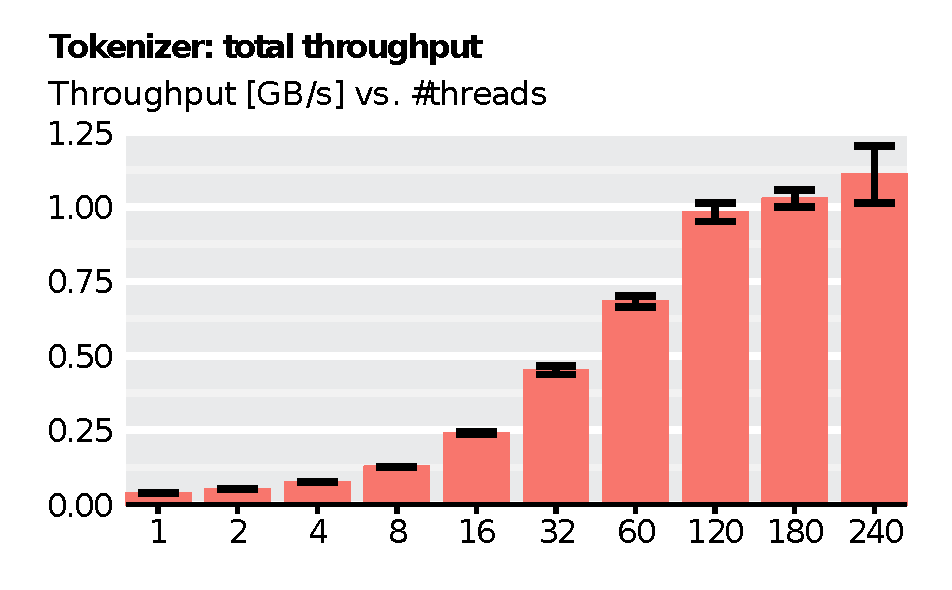
\includegraphics[scale=.45]{img/def/tokenizer_tp_total.eps}
    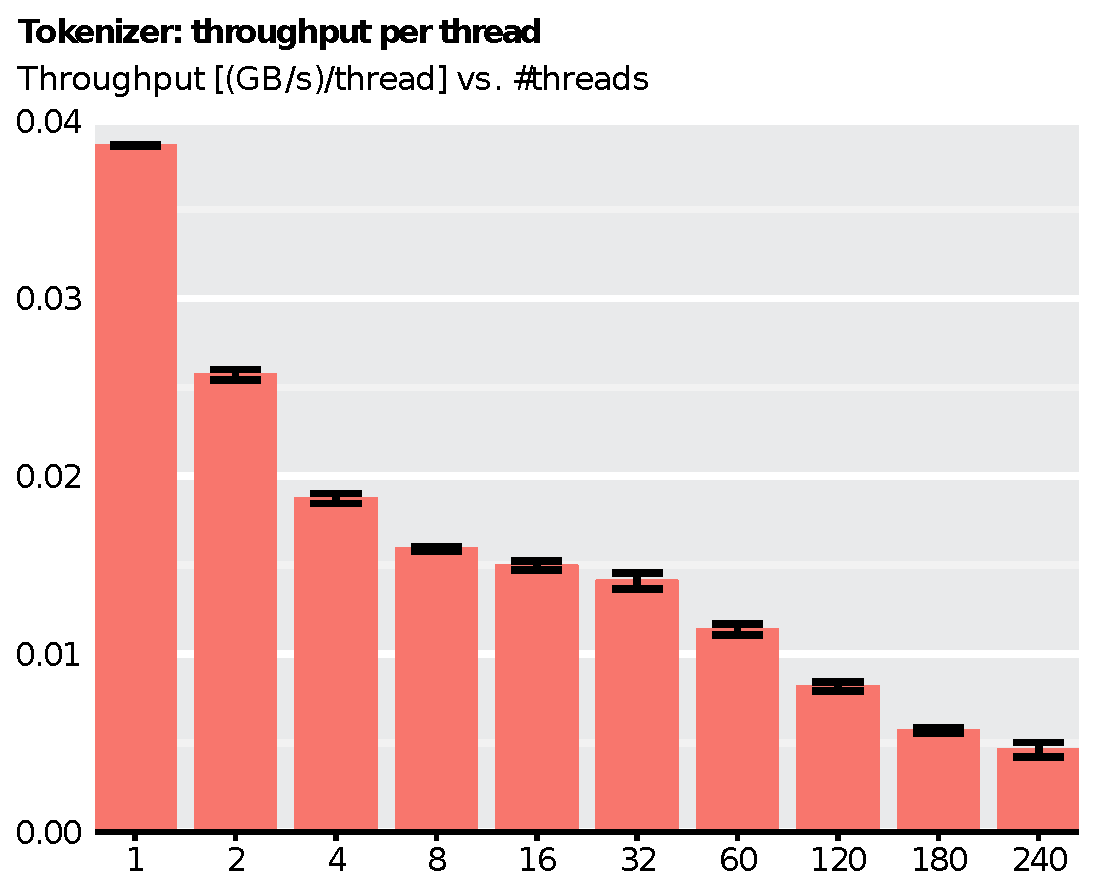
\includegraphics[scale=.45]{img/def/tokenizer_tp_per_thread.eps}
    \caption{Tokenizer Total Throughput and Throughput per Thread.}%
    \label{fig:tokenizertp}
\end{figure}

\begin{figure}
      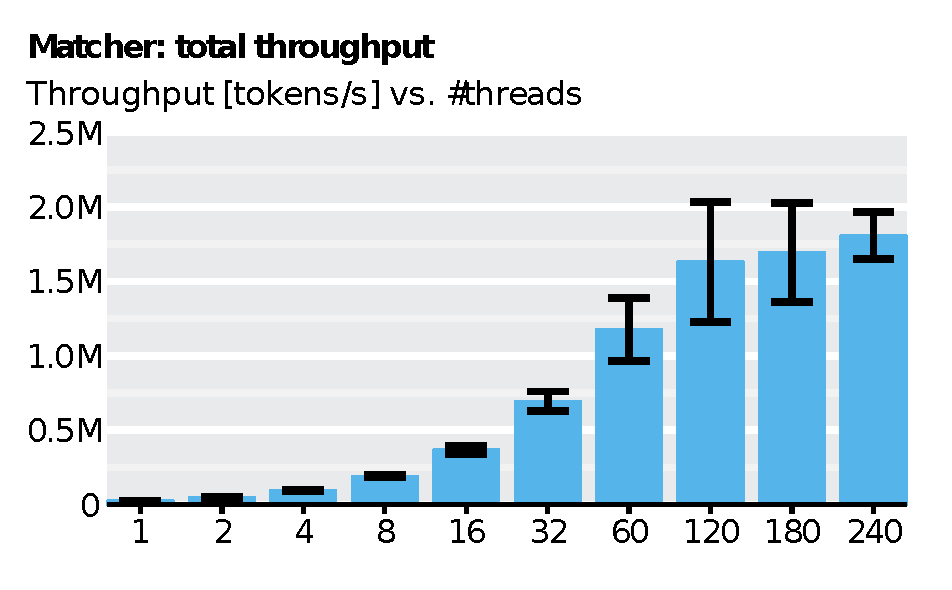
\includegraphics[scale=.45]{img/def/matcher_tp_total.eps}
      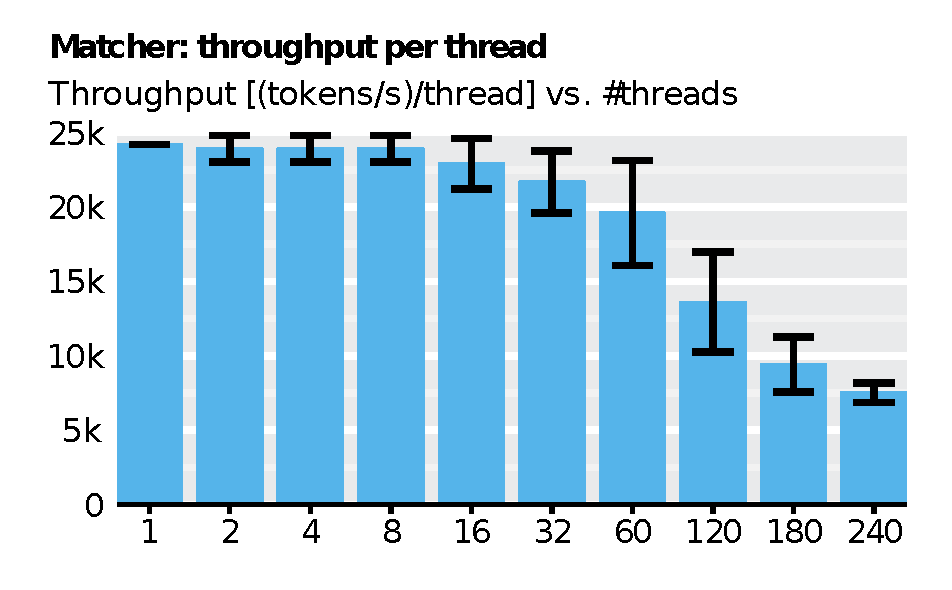
\includegraphics[scale=.45]{img/def/matcher_tp_per_thread.eps}
      \label{fig:matchertp}%
      \caption{Matcher: Total Throughput and Throughput per Thread.}
\end{figure}

\begin{figure}
    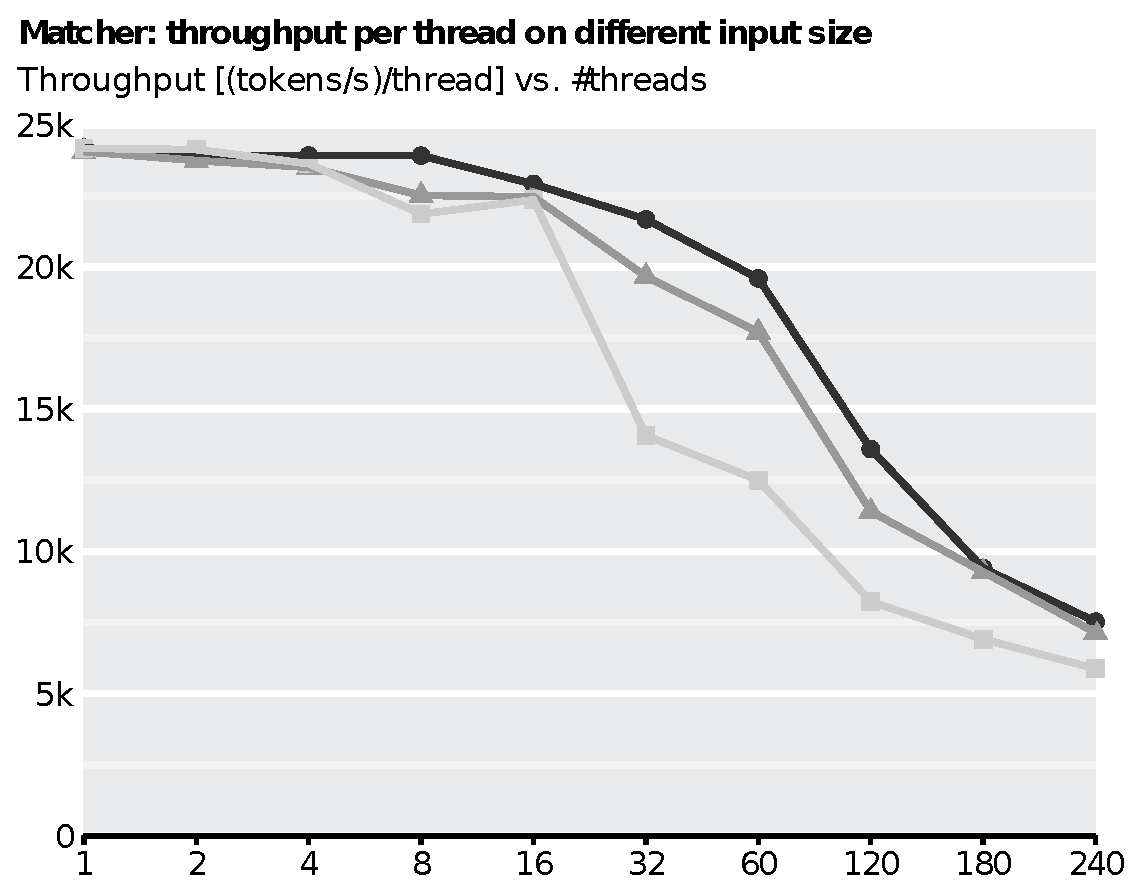
\includegraphics[scale=.45]{img/def/matcher_tp_compare.eps}
    \label{fig:tkmatchercomp}
    \caption{Throughput of matcher for different filesizes.}
\end{figure}

\begin{figure}
    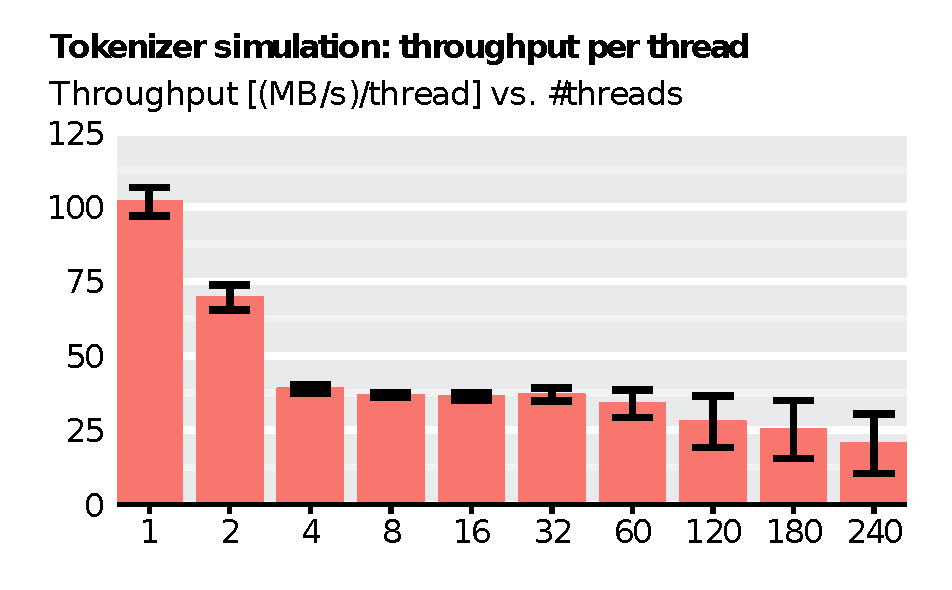
\includegraphics[scale=.45]{img/def/tokenizer_sim.eps} 
    \label{fig:tokenizersim}
    \caption{Experimental program simulating memory access pattern of the
    tokenizer.}
\end{figure}


In the following we present our experimental results. We only measured the
performance of the tokenizer and the matcher, as all other parts of the system
are I/O bound.

\mypar{Experimental Setup} The experiments were conducted on an Intel Xeon Phi
7120 coprocessor. This model contains 61 cores and 16 GB of GDDR5 memory with a
theoretical bandwidth of 352 GB/s. According to the documentation the Xeon Phi's
optimal computational power can be reached running two threads per core, i.e.
120 threads. For compilation the Intel Compiler version 15.0.0 20140723 was used
with the following flags: \verb;-fopenmp; \verb;-std=c++11; \verb;-mmic;
\verb;-Wall; \verb;-qopt-report3; \\ \verb;-qopt-report-phase=vec; \verb;-O3;.

To generate test data, we used the XML benchmark project XMark
\cite{Schmidt2002}. As input a 2 GB XML file was used containing 61'113'640
tags. 

\mypar{Results} First, we measured the performance of the tokenizer working
with 1 thread. Then we increased the number of threads to 2, 4, 8, 16, 32, 60,
120, 180 and 240.  Each experiment was run ten times. The results were built
with the average of these runs. Figure \ref{fig:tokenizertp} shows both, the
total throughput and the throughput per thread.

The experiments reveal clearly, that the throughput of the tokenizer increases
with the number of threads. While the benefits of more threads are significant
up to 120 threads, i.e. two threads per core, less performance can be gained
from 120 up to 240 threads.

Similarly, the matcher was tested with files of the sizes 2, 4 GB and 8 GB. For
each file 10 different experiments were run. In the first experiment one query
was used, corresponding to one thread, in the second 2 queries and the following
experiments 4, 8, 16, 32, 60, 120, 180 and 240 queries.  Again, the result is
the average of the runs. Figure \ref{fig:matchertp} shows the corresponding
results.

Since the file size alone does not reveal enough information about the
complexity, or the number of tokens in the XML data, the throughput for the
matcher is given in the number of tokens that are processed per second. Until up
to 60 queries there is no significant drop of the performance, while with 120
queries and more the throughput decreases significantly. Weak scaling is
observable for up to 60 threads. When the number of threads exceeds the number
of cores the performance suffers. This is in line with the observation Fang et
al. made in \cite{Fang14}.


To further asses the performance of the matcher, we included different file
sizes.

The sudden decrease of performance for 8 GB might be
due to the memory access pattern on the Xeon Phi, which becomes apparent, when
more threads operate at the same time on larger amount of data.  Pursuing
experiments that confirm this hypothesis would exceed the format of this report. 

A direct comparison of the processing time of the tokenizer and the matcher is
plotted in figure ~\ref{fig:tkmatchercomp}. The numbers represent the absolute
processing time of an XML file of 2 GB. Note that the number of threads for the
matcher is equal to the number of queries and is thus independent of the number
of threads for the tokenizer. One can see, that the processing time of the
matcher stays constant, even when increasing the numbers of queries being
processed, while decreasing drastically for the tokenizer when more threads are
provided.

The total throughput of the tokenizer and matcher running with 120 threads is
0.29 GBpss. This is far below the specified maximum memory bandwidth of 352
GBps. To make a realistic assessment of the maximally achievable throughput
we conducted an experiment with a dummy program which has a similar memory
access pattern as our tokenizer: A contiguous block of memory is read byte-wise
and every 80 bytes (based on the average number of tags per file) 10 bytes are
written to memory. The results are shown in Figure \ref{fig:tokenizersim}.
